Despite numerous efforts to decipher its origin (for example, \citealt{Wow_2024}), the "Wow!" signal  \citep{wow}  remains the most tantalizing unexplained radio signal today. This signal, seen in 1977 and rendered as "6EQUJ5" on the observatory printout, was unmistakably detected and aligned with the expected sidereal signal through the telescope beam, strongly implying an origin in deep space. At the time, the world had few transmitters in air or space, allowing the signal to stand out. However, in today's world, this momentous signal would be lost in the cacophony of our technological emissions that permeate the sky. Given all of this, the signal remains enigmatic to this day \citep{Saide_2023,Haqq_2025,Sheikh_2025}. Since it was only seen once, conclusive evidence of its origin has not been determined, which could have been anthropogenic or something more. Imagine going to a place where literally everything seen is of scientific interest and being able to explore it using modern technology that is far more advanced than the telescope used in 1977.   That is the promise of a lunar farside telescope.

Humanity is at a tipping point for conducting effective radio-astronomical observations from Earth. The ever-increasing use of wireless communication devices on the ground and in orbit means that nowhere on our planet, even remote locations with very low population density, is free of significant radio frequency interference (RFI). Although we have previously launched a small number of expensive ``Great Observatories'' into space, the increasing affordability and accessibility of space technology now make it feasible to deploy a large number of smaller telescopes. We are therefore at the edge of the transition from earth-based to space-based radio astronomy, born from the need to respond to changes in Earth's radio frequency environment, as well as the increased scope needed for scientific advancement. Making observations above the Earth's atmosphere and ionosphere also opens up observing windows inaccessible from Earth.

%Although terrestrial wireless communications seem to imply only negative implications for Earth-based radio astronomy, The same technology drivers  mean that smaller telescopes and experiments may cost-effectively be deployed to places with significantly less RFI, like the lunar farside. However, as this change occurs, the associated electronics, along with other active transmitters in space, will begin injecting 

However, in this transition to space, we risk injecting the same RFI into these new domains.  This is particularly true for the lunar farside, with its unique feature of always pointing away from the Earth providing essentially perfect shielding from the Earth \citep{MACCONE2019233,michaud2020lunar,heidmann2002}.
This makes it urgent to get well-designed sensors there as soon as possible to make early baseline measurements and conduct the unique science allowed only by its essentially RFI-free environment. The lunar farside represents a once-in-human history opportunity for quiet, high-quality observations, but this window will soon close as increasing scientific and political interest in lunar exploration brings new assets to the moon, as seen in Figure \ref{fig:missions}. Additionally, it also provides a unique opportunity to learn about the surface of the moon and to perform radio astronomy observations in off-world environments. 

\begin{figure}
    \centering
    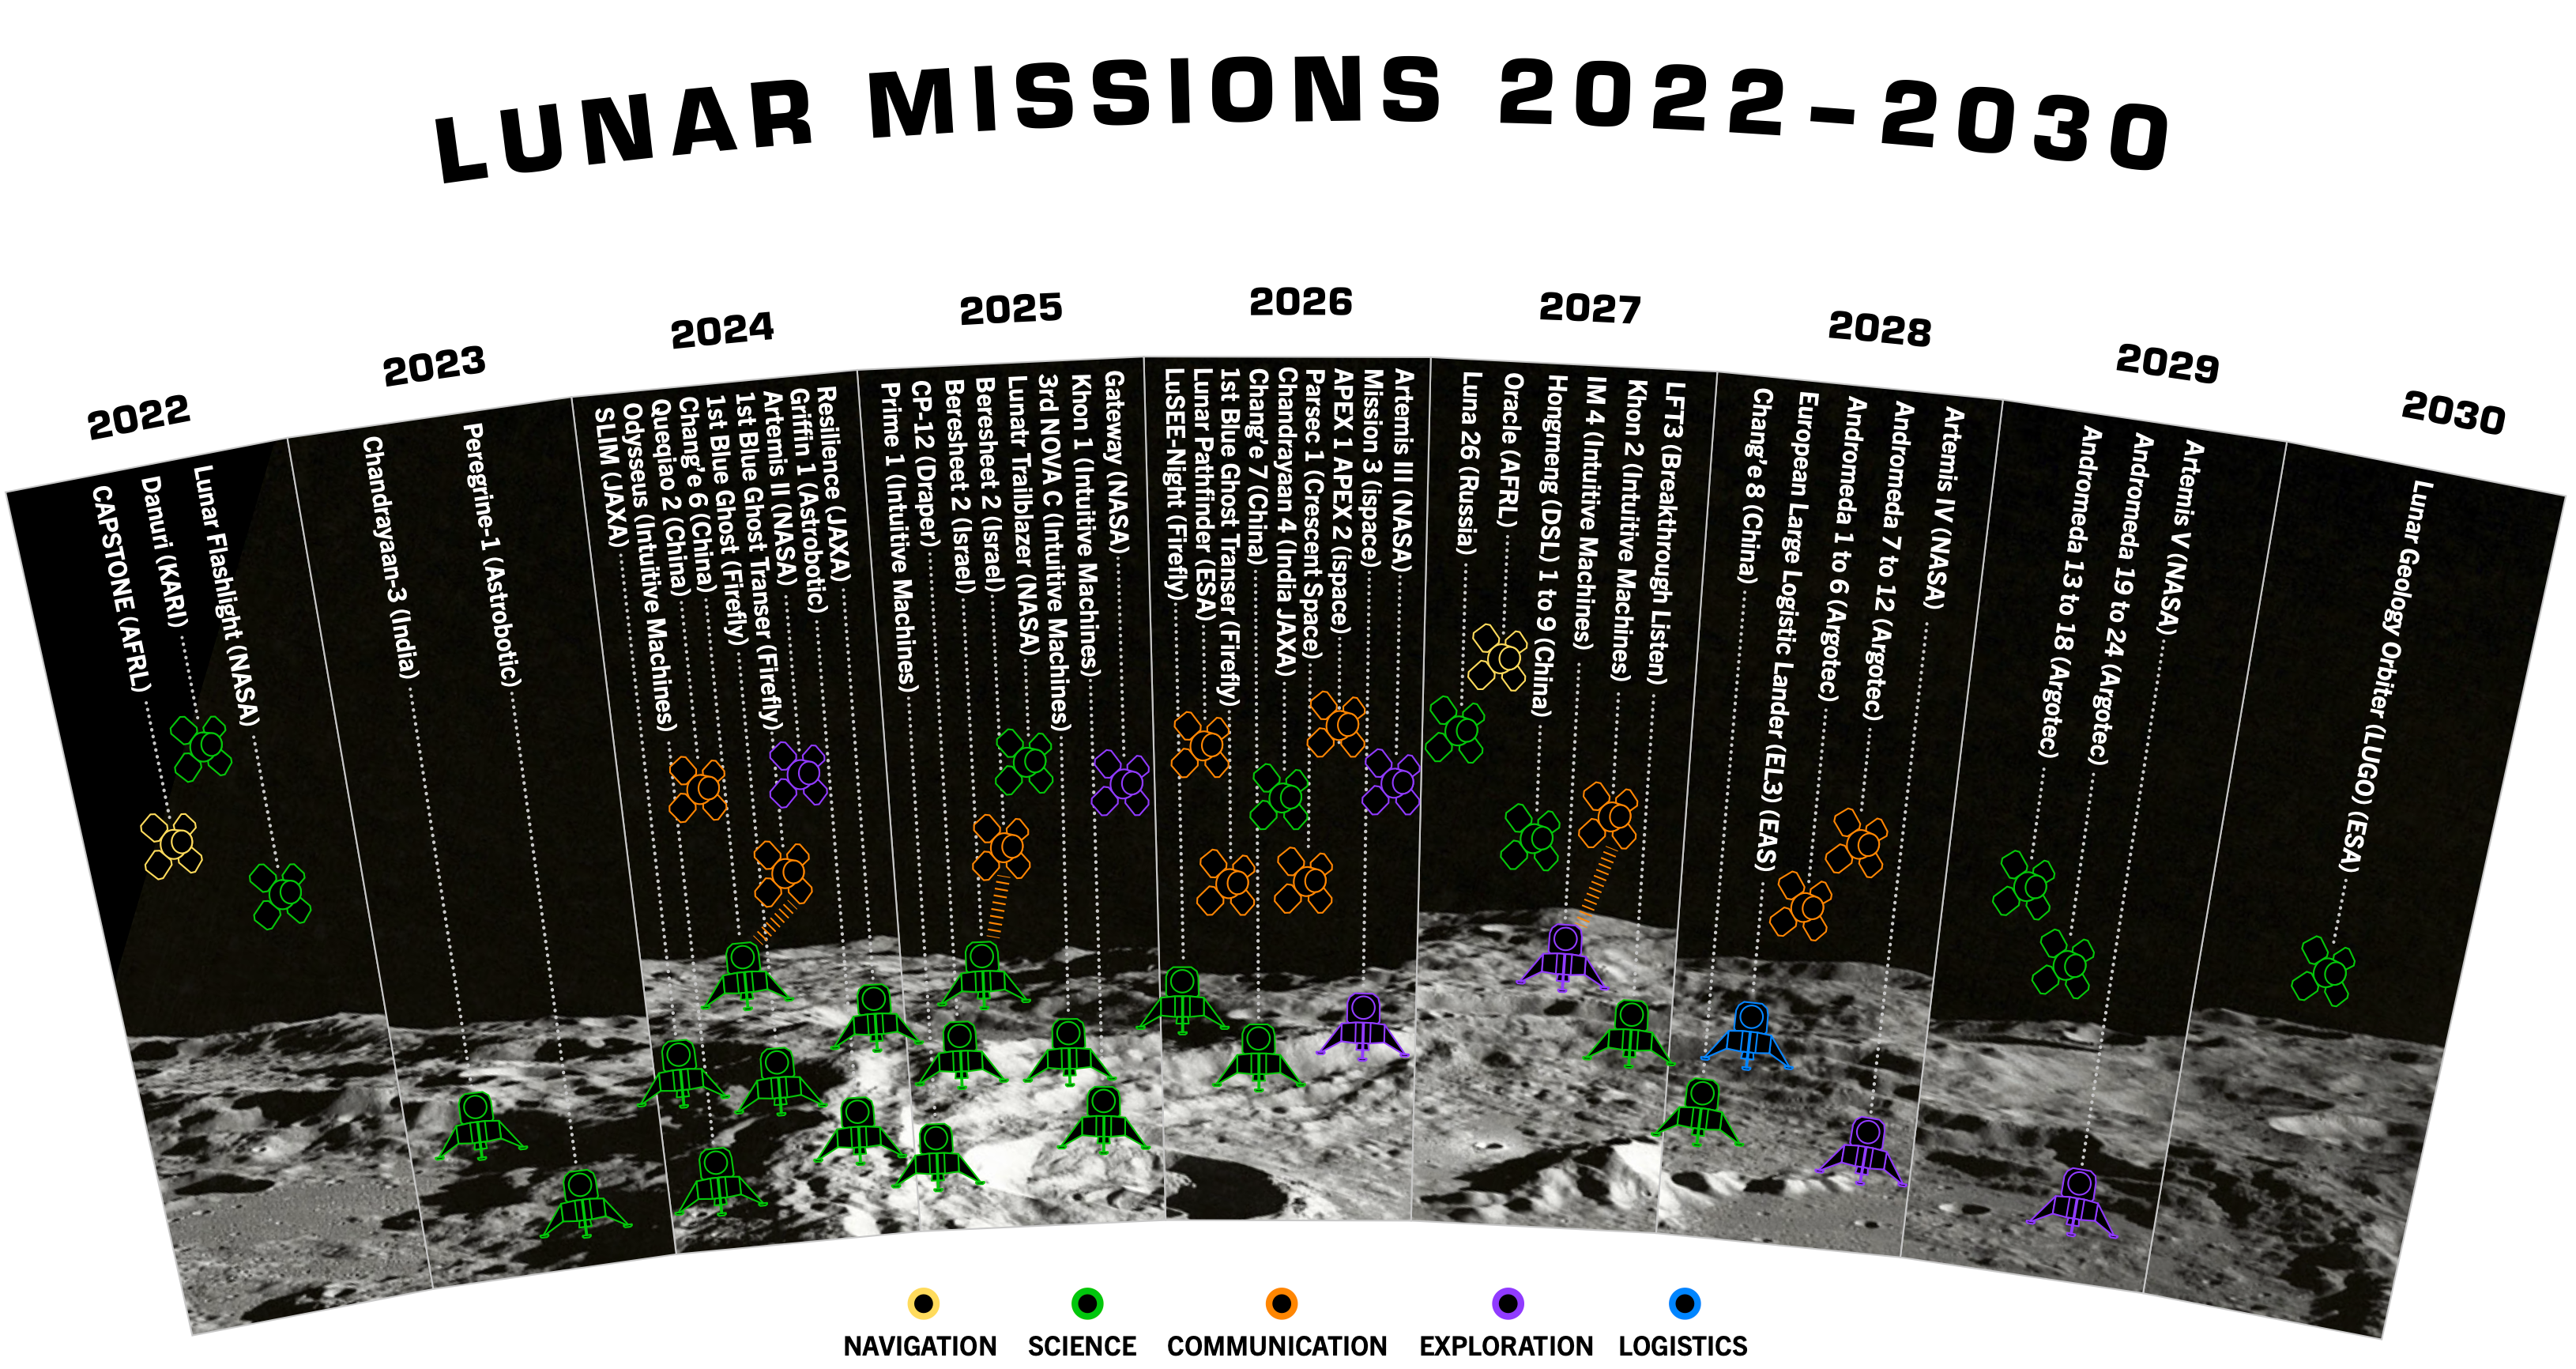
\includegraphics[width=\linewidth]{figures/missions.png}
    \caption{Graphic showing previous and planned cislunar missions with multiple objectives, as listed in the legend.    }
    \label{fig:missions}
\end{figure}

To act on this singular opportunity, we propose a radio telescope to be landed near the lunar antipode within five years to conduct these unique-in-history measurements. The telescope will comprise a suite of antennas and arrays designed to cover a wide range of frequencies and be of a scope that would allow for quick and cost-effective deployment in that timeframe.  Deploying and operating from the lunar farside introduces several system constraints. Key limitations include a total payload of approximately 100 kg, power consumption of 100 W during the lunar day, and data transmission of 100 GB/month back to Earth. Therefore, the system design and scientific objectives discussed in this document are subject to these system constraints.

The primary instrument is a UHF dual-pol multibeam phased array operating at $300-900$~MHz.  This band corresponds to a sensitivity maximum set by the increasing Galactic noise with decreasing frequency and the smaller collecting area for an array of this physical and fiscal scope as you increase frequency.  A smaller array operating at $900-2700$ MHz will allow a large band to be surveyed and will also allow the measurement of S-band communication signals from the Moon and potentially Mars.
Individual antennas will cover HF ($1-50$~MHz) and VHF in two bands, $60-110$~MHz and $150-250$~MHz. Note that at HF and VHF frequencies and for the scope of this mission, multiple antennas per band provide little to no benefit.  The mix of these receivers is unique to all other proposed missions and is well served by the stable and always shielded lunar farside location \citep{2021arXiv210305085B}.

Figure \ref{fig:freqbands} shows the frequency bands and their expected sensitivity, and Table \ref{tab:bandparam} provides an overview of the system.  During its mission lifetime, the telescope will observe most of the sky (see Fig. \ref{fig:fieldofview}) and conduct historical surveys in the solar system's most RFI-pristine environment before the presence of humanities' technology increases the radio frequency interference, even at this very remote place.  By the end of the decade it is likely that several dozen spacecraft will be orbiting the Moon, so time is limited.

\begin{figure}
    \centering
    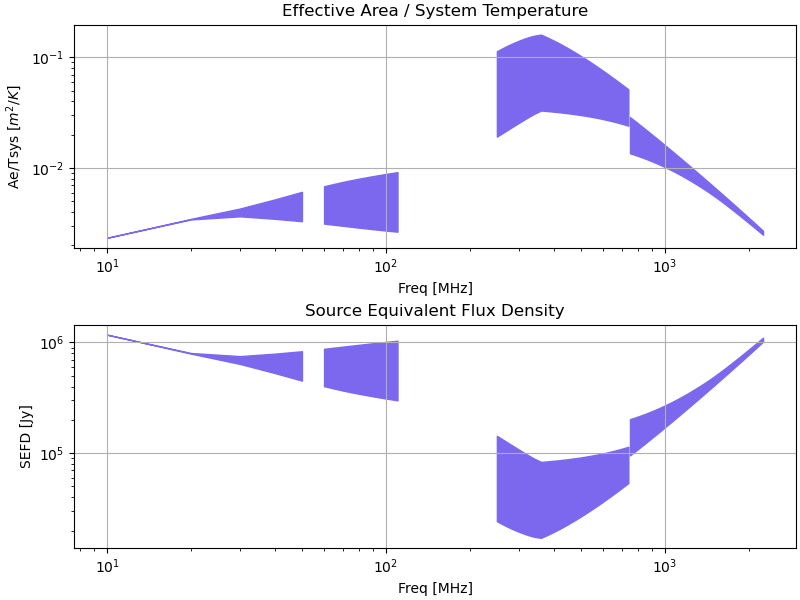
\includegraphics[width=0.75\linewidth]{figures/freqbands.png}
    \caption{Frequency bands of LFT3 and their associated sensitivity in terms of effective area over system temperature (top) and source equivalent flux density (bottom). The range stems from different fields over the varying sky temperatures due to Galactic emission and the plot is for the day-time powered system.}
    \label{fig:freqbands}
\end{figure}

\begin{figure}
    \centering
    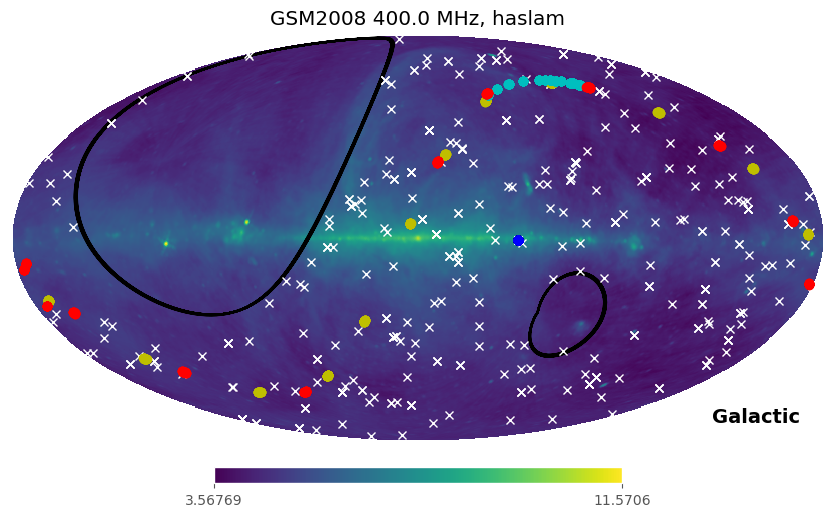
\includegraphics[width=0.95\linewidth]{figures/galaxy_plot.png}
    \caption{Graphic showing the field-of-view of LFT3 over the calendar year 2028 imposed over a graphic of Milky Way emission at 650 MHz \citep{2016ascl.soft03013P}.  The white points represent the stars within 10pc and the blue circle is Alpha Centauri. The yellow circles are the Sun's position as seen over the year. The red circles are Mars over that period and the cyan circles are Jupiter.  The interior region of the black shapes are outside the field-of-view.}
    \label{fig:fieldofview}
\end{figure}

\begin{figure}
    \centering
    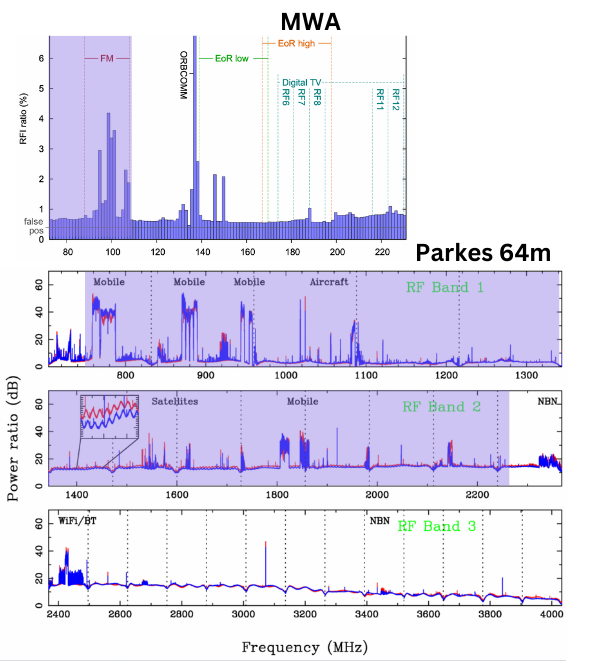
\includegraphics[width=0.75\linewidth]{figures/RFI_Plot.png}
    \caption{Figure showing the RFI environment at the Murchison Widefield Array (MWA; \citealt{Offringa_RFI}) and the Parkes 64m \citep{Hobbs_2020} telescopes. Highlighted are the regions proposed for use by the lunar telescope. This represent examples of the challenges ground-based observatories face when doing observations in the presence of RFI. The MWA site is government protected for radio astronomy, and even in this scenario RFI can still dominate certain regions of the spectrum and limiting the science outcomes.}
    \label{fig:RFI}
\end{figure}

In addition to the RFI considerations at radio frequencies, which can be extensive even in remote Earth locations, as shown in Figure \ref{fig:RFI}, there are other very significant scientific reasons for operating a radio telescope on the farside of the Moon. The ionosphere surrounding our planet creates a conducting medium through which electromagnetic radiation is impeded at frequencies below about 10\,MHz and distorted below about 30\,MHz\footnote{The impacted frequencies vary in time and place and are also a function of solar activity.} (e.g. \citealt{Zawdie_2017RS006256}) and for this reason low frequencies remain the last unexplored region of the electromagnetic spectrum.
Due to the absence of a tangible ionosphere on the moon, there are no technical barriers to studying physics at these new and unexplored frequencies. The primary motivations for targeting the lunar farside-- getting above the atmosphere and away from RFI-- are central to the design of the system. 

Note that RFI manifests itself in different ways, depending on its strength and an instrument's ability to handle it.  There are four basic RFI regimes\footnote{A new and emerging approach may be called "cooperative RF", whereby services coordinate their use -- this approach is being pursued by the US National Science Foundation in its National Radio Dynamic Zone research.}
(e.g. \citealt{Ellingson2005}, \citealt{selina2023detrimental}):
\begin{itemize}
    \item {\em Saturation}: Strong RFI that drives the receiver into saturation and creates problems throughout the band, effectively rendering it unusable.  This must be avoided at all costs by instrument design and operational constraints. Avoidance is increasingly difficult to achieve due to increasing RFI sources, such as large satellite constellations.
    \item {\em Coherent mitigation}: If the receiver is not overly saturated with strong RFI and if the characteristics of the interferer are known or retrievable, it is possible, in some cases, to mitigate by subtraction or suppression of the interferer.  This has largely been in the research rather than operational realm given its difficulty and its effect on the science data.  It may be useful in the future for certain science goals, such as detecting transients such as pulsars and fast radio bursts (FRBs), or with widely separated coherent receivers.  Another technique for arrays is to steer nulls towards interferers in known directions.
    \item {\em Identification and excision}:  As in the case above, if the receiver is not in significant compression and if the RFI can be identified (taking into account harmonics), it may be removed or ``flagged'', with a resultant loss of data.  This is by far the dominant technique used in radio astronomy.  This technique generally allows some science to proceed; however, it provides a scientific limit and a loss of discovery opportunity.
    \item {\em Low-level}:  This is the insidious presence of low-level RFI that is below the threshold of identification and excision.  It provides a low-level noise floor that is essentially unknowable and is a particular issue for extremely high-sensitivity cosmological global experiments. Observing at these frequencies without low-level RFI is a unique aspect of the lunar farside.
\end{itemize}
Lunar farside observations are currently free from all of these aspects of RFI, representing our only chance of observing without the low-level RFI noise that impacts sensitive radio astronomical measurements in all other environments.

When considering this endeavor, some other factors should be considered:
%\vspace{-0.3cm}
\begin{itemize}
    \item At low frequencies, the system temperature will be dominated by Galactic noise and impulsive events will be affected by scattering and dispersion. Any civilization generating a beacon will be aware of this constraint regardless of where they are located in the Galaxy, which tends to discourage arguments for low-frequency SETI.  However, this is the last unexplored region of the electromagnetic spectrum and should be thoroughly observed.
    \item Having the widest possible absolute bandwidth and largest feasible field-of-view will maximize the possibility for serendipitous discoveries, particularly of rare events.
    \item The possibility of initial discovery of technosignatures in the aforementioned bands with Earth-based telescopes is drowned out by ``anthropogenic technosignatures'' aka RFI.  The lunar farside should be completely devoid of this for at least 5 years.
   \item LuSEE-Night will operate from the lunar farside at radio frequencies (0.1-50MHz) that are below the Earth's ionospheric cut-off to make radio astronomical observations impossible, which can be augmented by this telescope.
    \item An all-sky monitor from the lunar surface will give an unprecedented view of bright but rare transient events, including those obscured by the atmosphere and RFI from Earth.
    \item Our window for collecting interference-free legacy spectra is brief. By 2030, more than a dozen satellites are expected to orbit the Moon, significantly increasing RFI on the lunar farside.
    \item The unique scientific payload on the lunar farside is always shielded from Earth's RFI and has longer sky dwell times due to the slow lunar rotation.
\end{itemize}

We note that an observatory on the farside of the moon has no visibility of Earth, and thus would have limited use for military or intelligence purposes, emphasizing its exclusively peaceful, scientific mission. Potential science cases for bringing this telescope to life are outlined in the next section, followed by a discussion of the payload and operational model.  A discussion of other potential telescope locations and options is then discussed, demonstrating the unique qualities of the lunar farside for this mission.